\hypertarget{operator}{%
\chapter{演算子}\label{operator}}\index{えんざんし@演算子}
\thispagestyle{frontheadings}

演算子はよく利用する演算処理を記号などで表現したものです。
たとえば、足し算をする \texttt{+}
も演算子の一種です。これ以外にも演算子には多くの種類があります。

演算子は演算する対象を持ちます。この演算子の対象のことを\textbf{\textgt{被演算子(オペランド)}}\index{ひえんざんし@被演算子}\index{おぺらんど@オペランド}と呼びます。

次のコードでは、\texttt{+}演算子が値同士を足し算する加算演算を行っています。
このとき、\texttt{+}演算子の対象となっている\texttt{1}と\texttt{2}という2つの値がオペランドです。

\begin{lstlisting}
1 + 2;
\end{lstlisting}

このコードでは\texttt{+}演算子に対して、前後に合計2つのオペランドがあります。
このように、2つのオペランドを取る演算子を\textbf{\textgt{二項演算子}}\index{にこうえんざんし@二項演算子}と呼びます。

\begin{lstlisting}
// 二項演算子とオペランドの関係
左オペランド 演算子 右オペランド
\end{lstlisting}

また、1つの演算子に対して1つのオペランドだけを取るものもあります。
たとえば、数値をインクリメントする\texttt{++}演算子は、次のように前後どちらか一方にオペランドを置きます。

\begin{lstlisting}
let num = 1;
num++;
// または
++num;
\end{lstlisting}

このように、1つのオペランドを取る演算子を\textbf{\textgt{単項演算子}}\index{たんこうえんざんし@単項演算子}と呼びます。
単項演算子と二項演算子で同じ記号を使うことがあるため、呼び方を変えています。

この章では、演算子ごとにそれぞれの処理について学んでいきます。
また、演算子の中でも比較演算子は、JavaScriptでも特に挙動が理解しにくい\textbf{\textgt{暗黙的な型変換}}\index{あんもくてきなかたへんかん@暗黙的な型変換}という問題と密接な関係があります。
そのため、演算子をひととおり見た後に、暗黙的な型変換と明示的な型変換について学んでいきます。

演算子の種類は多いため、すべての演算子の動作をここで覚える必要はありません。
必要となったタイミングで、改めてその演算子の動作を見るのがよいでしょう。

\hypertarget{binary-operator}{%
\section{二項演算子}\label{binary-operator}}\index{にこうえんざんし@二項演算子}

四則演算など基本的な二項演算子を見ていきます。

\hypertarget{plus-operator}{%
\subsection{\texorpdfstring{プラス演算子(\texttt{+})}{プラス演算子(+)}}\label{plus-operator}}\index{ぷらすえんざんし@プラス演算子}\index{+@\texttt{+}}

2つの数値を加算する演算子です。

\begin{lstlisting}
console.log(1 + 1); // => 2
\end{lstlisting}

JavaScriptでは、数値は内部的にIEEE
754方式の浮動小数点数として表現されています (
\hyperlink{data-type-and-literal}{「データ型とリテラル」}の章を参照)。
そのため、整数と浮動小数点数の加算もプラス演算子で行えます。

\begin{lstlisting}
console.log(10 + 0.5); // => 10.5
\end{lstlisting}

\hypertarget{string-combination-operator}{%
\subsection{\texorpdfstring{文字列結合演算子(\texttt{+})}{文字列結合演算子(+)}}\label{string-combination-operator}}\index{もじれつけつごうえんざんし@文字列結合演算子}\index{+@\texttt{+}}

数値の加算に利用したプラス演算子(\texttt{+})は、文字列の結合に利用できます。

文字列結合演算子(\texttt{+})は、2つの文字列を結合した文字列を返します。

\begin{lstlisting}
const value = "文字列" + "結合";
console.log(value); // => "文字列結合"
\end{lstlisting}

つまり、プラス演算子(\texttt{+})は数値同士と文字列同士の演算をします。

\hypertarget{minus-operator}{%
\subsection{\texorpdfstring{マイナス演算子(\texttt{-})}{マイナス演算子(-)}}\label{minus-operator}}\index{まいなすえんざんし@マイナス演算子}\index{-@\texttt{-}}

2つの数値を減算する演算子です。左オペランドから右オペランドを減算した値を返します。

\begin{lstlisting}
console.log(1 - 1); // => 0
console.log(10 - 0.5); // => 9.5
\end{lstlisting}

\hypertarget{multiplication-operator}{%
\subsection{\texorpdfstring{乗算演算子(\texttt{*})}{乗算演算子(*)}}\label{multiplication-operator}}\index{じょうざんえんざんし@乗算演算子}\index{*@\texttt{*}}

2つの数値を乗算する演算子です。

\begin{lstlisting}
console.log(2 * 8); // => 16
console.log(10 * 0.5); // => 5
\end{lstlisting}

\hypertarget{division-operator}{%
\subsection{\texorpdfstring{除算演算子(\texttt{/})}{除算演算子(/)}}\label{division-operator}}\index{じょざんえんざんし@除算演算子}\index{/@\texttt{/}}

2つの数値を除算する演算子です。左オペランドを右オペランドで除算した値を返します。

\begin{lstlisting}
console.log(8 / 2); // => 4
console.log(10 / 0.5); // => 20
\end{lstlisting}

ただし、任意の数値を\texttt{0}で除算した結果は、無限大を表す数値である\texttt{Infinity}となります。

\begin{lstlisting}
console.log(10 / 0); // => Infinity
\end{lstlisting}

\hypertarget{modulus-operator})}{剰余演算子(\%)}}\label{modulus-operator}}\index{じょうよえんざんし@剰余演算子}\index{\%@\texttt{\%}}

2つの数値を除算したあまりを求める演算子です。左オペランドを右オペランドで除算したあまりを返します。

\begin{lstlisting}
console.log(8 % 2); // => 0
console.log(9 % 2); // => 1
console.log(10 % 0.5); // => 0
console.log(10 % 4.5); // => 1
\end{lstlisting}

\hypertarget{pow-operator}{%
\subsection[べき乗演算子(\texttt{**})]{べき乗演算子(\texttt{**})\protect\icon{fig/es2016.eps}}\label{pow-operator}}\index{べきじょうえんざんし@べき乗演算子}\index{**@\texttt{**}}

2つの数値のべき乗を求める演算子です。
左オペランドを右オペランドでべき乗した値を返します。

\begin{lstlisting}
// べき乗演算子(ES2016)で2の4乗を計算
console.log(2 ** 4); // => 16
\end{lstlisting}

べき乗演算子と同じ動作をする\texttt{Math.pow}メソッドがあります。

\begin{lstlisting}
console.log(Math.pow(2, 4)); // => 16
\end{lstlisting}

べき乗演算子はES2016で後から追加された演算子であるため、関数と演算子がそれぞれ存在しています。
一方、他の二項演算子は演算子が先に存在していたため、\texttt{Math}には対応するメソッドがありません。

\hypertarget{unary-operator}{%
\section{単項演算子(算術)}\label{unary-operator}}\index{たんこうえんざんし@単項演算子}\index{さんじゅつ@算術}

単項演算子は、1つのオペランドを受け取って処理する演算子です。

\hypertarget{unary-plus-operator}{%
\subsection{\texorpdfstring{単項プラス演算子(\texttt{+})}{単項プラス演算子(+)}}\label{unary-plus-operator}}\index{たんこうぷらすえんざんし@単項プラス演算子}\index{+@\texttt{+}}

単項演算子の\texttt{+}はオペランドを数値に変換します。

次のコードでは、数値の\texttt{1}を数値へ変換するため、結果は変わらず数値の\texttt{1}です。
\texttt{+数値}のように数値に対して、単項プラス演算子をつけるケースはほぼ無いでしょう。

\begin{lstlisting}
console.log(+1); // => 1
\end{lstlisting}

また、単項プラス演算子は、数値以外も数値へと変換します。
次のコードでは、数字(文字列)を数値へ変換しています。

\begin{lstlisting}
console.log(+"1"); // => 1
\end{lstlisting}

一方、数値に変換できない文字列などは\texttt{NaN}\index{NaN@\texttt{NaN}}という特殊な値へと変換されます。

\begin{lstlisting}
// 数値ではない文字列はNaNという値に変換される
console.log(+"文字列"); // => NaN
\end{lstlisting}

\texttt{NaN}は``Not-a-Number''の略称で、数値ではないがNumber型の値を表現しています。
\texttt{NaN}はどの値とも(NaN自身に対しても)一致しない特性があり、\texttt{Number.isNaN}\index{Number.isNaN@\texttt{Number.isNaN}}メソッドを使うことで\texttt{NaN}の判定を行えます。

\begin{lstlisting}
// 自分自身とも一致しない
console.log(NaN === NaN); // => false
// Number型である
console.log(typeof NaN); // => "number"
// Number.isNaNでNaNかどうかを判定
console.log(Number.isNaN(NaN)); // => true
\end{lstlisting}

しかし、単項プラス演算子は文字列から数値への変換に使うべきではありません。
なぜなら、\texttt{Number}コンストラクタ関数や\texttt{parseInt}関数などの明示的な変換方法が存在するためです。
詳しくは「\hyperlink{implicit-coercion}{暗黙的な型変換}」の章で解説します。

\hypertarget{unary-minus-operator}{%
\subsection{\texorpdfstring{単項マイナス演算子(\texttt{-})}{単項マイナス演算子(-)}}\label{unary-minus-operator}}\index{たんこうまいなすえんざんし@単項マイナス演算子}\index{-@\texttt{-}}

単項マイナス演算子はマイナスの数値を記述する場合に利用します。

たとえば、マイナスの1という数値を \texttt{-1}
と書くことができるのは、単項マイナス演算子を利用しているからです。

\begin{lstlisting}
console.log(-1); // => -1
\end{lstlisting}

また、単項マイナス演算子はマイナスの数値を反転できます。
そのため、``マイナスのマイナスの数値''はプラスの数値となります。

\begin{lstlisting}
console.log(-(-1)); // => 1
\end{lstlisting}

単項マイナス演算子も文字列などを数値へ変換します。

\begin{lstlisting}
console.log(-"1"); // => -1
\end{lstlisting}

また、数値へ変換できない文字列などをオペランドに指定した場合は、\texttt{NaN}という特殊な値になります。
そのため、単項プラス演算子と同じく、文字列から数値への変換に単項マイナス演算子を使うべきではありません。

\begin{lstlisting}
console.log(-"文字列"); // => NaN
\end{lstlisting}

\hypertarget{increment-operator}{%
\subsection{\texorpdfstring{インクリメント演算子(\texttt{++})}{インクリメント演算子(++)}}\label{increment-operator}}\index{いんくりめんとえんざんし@インクリメント演算子}\index{++@\texttt{++}}

インクリメント演算子(\texttt{++})は、オペランドの数値を\texttt{+1}する演算子です。
オペランドの前後どちらかにインクリメント演算子を置くことで、オペランドに対して値を\texttt{+1}した値を返します。

\begin{lstlisting}
let num = 1;
num++;
console.log(num); // => 2
// 次のようにした場合と結果は同じ
// num = num + 1;
\end{lstlisting}

インクリメント演算子(\texttt{++})は、オペランドの前後どちらに置くかによって評価の順番が異なります。

後置インクリメント演算子(\texttt{num++})は、次のような順で処理が行われます。

\begin{enumerate}
\def\labelenumi{\arabic{enumi}.}
\item
  \texttt{num}の評価結果を返す
\item
  \texttt{num}に対して\texttt{+1}する
\end{enumerate}

そのため、\texttt{num++}が返す値は\texttt{+1}する前の値となります。

\begin{lstlisting}
let x = 1;
console.log(x++); // => 1
console.log(x);   // => 2
\end{lstlisting}

一方、前置インクリメント演算子(\texttt{++num})は、次のような順で処理が行われます。

\begin{enumerate}
\def\labelenumi{\arabic{enumi}.}
\item
  \texttt{num}に対して\texttt{+1}する
\item
  \texttt{num}の評価結果を返す
\end{enumerate}

そのため、\texttt{++num}が返す値は\texttt{+1}した後の値となります。

\begin{lstlisting}
let x = 1;
console.log(++x); // => 2
console.log(x);   // => 2
\end{lstlisting}

この2つの使い分けが必要となる場面は多くありません。
そのため、評価の順番が異なることだけを覚えておけば問題ないと言えます。

\hypertarget{decrement-operator}{%
\subsection{\texorpdfstring{デクリメント演算子(\texttt{-\/-})}{デクリメント演算子(-\/-)}}\label{decrement-operator}}\index{でくりめんとえんざんし@デクリメント演算子}\index{--@\texttt{-\/-}}

デクリメント演算子(\texttt{-\/-})は、オペランドの数値を\texttt{-1}する演算子です。

\begin{lstlisting}
let num = 1;
num--;
console.log(num); // => 0
// 次のようにした場合と結果は同じ
// num = num - 1;
\end{lstlisting}

デクリメント演算子は、インクリメント演算子と同様に、オペランドの前後のどちらかに置くことができます。
デクリメント演算子も、前後どちらに置くかで評価の順番が変わります。

\begin{lstlisting}
// 後置デクリメント演算子
let x = 1;
console.log(x--); // => 1
console.log(x);   // => 0
// 前置デクリメント演算子
let y = 1;
console.log(--y); // => 0
console.log(y);   // => 0
\end{lstlisting}

\hypertarget{comparison-operator}{%
\section{比較演算子}\label{comparison-operator}}\index{ひかくえんざんし@比較演算子}

比較演算子はオペランド同士の値を比較し、真偽値を返す演算子です。

\hypertarget{strict-equal-operator}{%
\subsection{\texorpdfstring{厳密等価演算子(\texttt{===})}{厳密等価演算子(===)}}\label{strict-equal-operator}}\index{げんみつとうかえんざんし@厳密等価演算子}\index{===@\texttt{===}}

厳密等価演算子は、左右の2つのオペランドを比較します。
同じ型で同じ値である場合に、\texttt{true}を返します。

\begin{lstlisting}
console.log(1 === 1); // => true
console.log(1 === "1"); // => false
\end{lstlisting}

また、オペランドがどちらもオブジェクトであるときは、
オブジェクトの参照が同じである場合に、\texttt{true}を返します。

次のコードでは、空のオブジェクトリテラル(\texttt{\{\}})同士を比較しています。
オブジェクトリテラルは、新しいオブジェクトを作成します。
そのため、異なるオブジェクトを参照する変数を\texttt{===}で比較すると\texttt{false}を返します。

\begin{lstlisting}
// {} は新しいオブジェクトを作成している
const objA = {};
const objB = {};
// 生成されたオブジェクトは異なる参照となる
console.log(objA === objB); // => false
// 同じ参照を比較している場合
console.log(objA === objA); // => true
\end{lstlisting}

\hypertarget{strict-not-equal-operator}{%
\subsection{\texorpdfstring{厳密不等価演算子(\texttt{!==})}{厳密不等価演算子(!==)}}\label{strict-not-equal-operator}}\index{げんみつふとうかえんざんし@厳密不等価演算子}\index{"!==@\texttt{"!==}}

厳密不等価演算子は、左右の2つのオペランドを比較します。
異なる型または異なる値である場合に、\texttt{true}を返します。

\begin{lstlisting}
console.log(1 !== 1); // => false
console.log(1 !== "1"); // => true
\end{lstlisting}

\texttt{===}を反転した結果を返す演算子となります。

\hypertarget{equal-operator}{%
\subsection{\texorpdfstring{等価演算子(\texttt{==})}{等価演算子(==)}}\label{equal-operator}}\index{とうかえんざんし@等価演算子}\index{==@\texttt{==}}

等価演算子(\texttt{==})は、2つのオペランドを比較します。
同じデータ型のオペランドを比較する場合は、厳密等価演算子(\texttt{===})と同じ結果になります。

\begin{lstlisting}
console.log(1 == 1); // => true
console.log("str" == "str"); // => true
console.log("JavaScript" == "ECMAScript"); // => false
// オブジェクトは参照が一致しているならtrueを返す
// {} は新しいオブジェクトを作成している
const objA = {};
const objB = {};
console.log(objA == objB); // => false
console.log(objA == objA); // => true
\end{lstlisting}

しかし、等価演算子(\texttt{==})はオペランド同士が異なる型の値であった場合に、
同じ型となるように\textbf{\textgt{暗黙的な型変換}}\index{あんもくてきなかたへんかん@暗黙的な型変換}をしてから比較します。

そのため、次のような、見た目からは結果を予測できない挙動が多く存在します。

\begin{lstlisting}
// 文字列を数値に変換してから比較
console.log(1 == "1"); // => true
// "01"を数値にすると1となる
console.log(1 == "01"); // => true
// 真偽値を数値に変換してから比較
console.log(0 == false); // => true
// nullの比較はfalseを返す
console.log(0 == null); // => false
// nullとundefinedの比較は常にtrueを返す
console.log(null == undefined); // => true
\end{lstlisting}

意図しない挙動となることがあるため、暗黙的な型変換が行われる等価演算子(\texttt{==})を使うべきではありません。
代わりに、厳密等価演算子(\texttt{===})を使い、異なる型を比較したい場合は明示的に型を合わせるべきです。

例外的に、等価演算子(\texttt{==})が使われるケースとして、\texttt{null}と\texttt{undefined}の比較があります。

次のように、比較したいオペランドが \texttt{null} または
\texttt{undefined} であることを判定したい場合に、
厳密等価演算子(\texttt{===})では二度比較する必要があります。
等価演算子(\texttt{==})では\texttt{null}と\texttt{undefined}の比較結果は\texttt{true}となるため、一度の比較でよくなります。

\begin{lstlisting}
const value = undefined; /* または null */
// === では2つの値と比較しないといけない
if (value === null || value === undefined) {
    console.log("valueがnullまたはundefinedである場合の処理");
}
// == では null と比較するだけでよい
if (value == null) {
    console.log("valueがnullまたはundefinedである場合の処理");
}
\end{lstlisting}

このように等価演算子(\texttt{==})を使う例外的なケースはありますが、
等価演算子(\texttt{==})は\hyperlink{implicit-coercion}{暗黙的な型変換}をするため、バグを引き起こしやすいです。
そのため、仕組みを理解するまでは常に厳密等価演算子(\texttt{===})を利用することを推奨します。

\hypertarget{not-equal-operator}{%
\subsection{\texorpdfstring{不等価演算子(\texttt{!=})}{不等価演算子(!=)}}\label{not-equal-operator}}\index{ふとうかえんざんし@不等価演算子}\index{"!=@\texttt{"!=}}

不等価演算子(\texttt{!=})は、2つのオペランドを比較し、等しくないなら\texttt{true}を返します。

\begin{lstlisting}
console.log(1 != 1); // => false
console.log("str" != "str"); // => false
console.log("JavaScript" != "ECMAScript"); // => true
console.log(true != true);// => false
// オブジェクトは参照が一致していないならtrueを返す
const objA = {};
const objB = {};
console.log(objA != objB); // => true
console.log(objA != objA); // => false
\end{lstlisting}

不等価演算子も、等価演算子(\texttt{==})と同様に異なる型のオペランドを比較する際に、暗黙的な型変換\index{あんもくてきなかたへんかん@暗黙的な型変換}をしてから比較します。

\begin{lstlisting}
console.log(1 != "1"); // => false
console.log(0 != false); // => false
console.log(0 != null); // => true
console.log(null != undefined); // => false
\end{lstlisting}

そのため、不等価演算子(\texttt{!=})は、利用するべきではありません。
代わりに暗黙的な型変換をしない厳密不等価演算子(\texttt{!==})を利用します。

\hypertarget{more-than}{%
\subsection{\texorpdfstring{大なり演算子/より大きい(\texttt{\textgreater{}})}{大なり演算子/より大きい(\textgreater{})}}\label{more-than}}\index{だいなりえんざんし@大なり演算子}\index{>@\texttt{\textgreater}}

大なり演算子は、左オペランドが右オペランドより大きいならば、\texttt{true}を返します。

\begin{lstlisting}
console.log(42 > 21); // => true
console.log(42 > 42); // => false
\end{lstlisting}

\hypertarget{more-than-equal}{%
\subsection{\texorpdfstring{大なりイコール演算子/以上(\texttt{\textgreater{}=})}{大なりイコール演算子/以上(\textgreater{}=)}}\label{more-than-equal}}\index{だいなりいこーるえんざんし@大なりイコール演算子}\index{>=@\texttt{\textgreater{}=}}

大なりイコール演算子は、左オペランドが右オペランドより大きいまたは等しいならば、\texttt{true}を返します。

\begin{lstlisting}
console.log(42 >= 21); // => true
console.log(42 >= 42); // => true
console.log(42 >= 43); // => false
\end{lstlisting}

\hypertarget{less-than}{%
\subsection{\texorpdfstring{小なり演算子/より小さい(\texttt{\textless{}})}{小なり演算子/より小さい(\textless{})}}\label{less-than}}\index{しょうなりえんざんし@小なり演算子}\index{<@\texttt{\textless}}

小なり演算子は、左オペランドが右オペランドより小さいならば、\texttt{true}を返します。

\begin{lstlisting}
console.log(21 < 42); // => true
console.log(42 < 42); // => false
\end{lstlisting}

\hypertarget{less-than-equal}{%
\subsection{\texorpdfstring{小なりイコール演算子/以下(\texttt{\textless{}=})}{小なりイコール演算子/以下(\textless{}=)}}\label{less-than-equal}}\index{しょうなりいこーるえんざんし@小なりイコール演算子}\index{<=@\texttt{\textless{}=}}

小なりイコール演算子は、左オペランドが右オペランドより小さいまたは等しいならば、\texttt{true}を返します。

\begin{lstlisting}
console.log(21 <= 42); // => true
console.log(42 <= 42); // => true
console.log(43 <= 42); // => false
\end{lstlisting}

\hypertarget{bit-operator}{%
\section{ビット演算子}\label{bit-operator}}\index{びっとえんざんし@ビット演算子}

ビット演算子では、オペランドである数値を符号付き32ビット整数(\texttt{0}と\texttt{1}からなる32個のビットの集合)として扱います。

たとえば、\texttt{1}という数値は符号付き32ビット整数のビットでは、\texttt{00000000000000000000000000000001}として表現されます。
わかりやすく4ビットごとに区切ると\texttt{0000\_0000\_0000\_0000\_0000\_0000\_0000\_0001}のような32ビットの集合となります。
符号付き32ビット整数では、先頭の最上位ビット(一番左のビット)は符号を表し、\texttt{0}の場合は正の値、\texttt{1}の場合は負の値であることを示しています。

\begin{figure}[h]
\centering
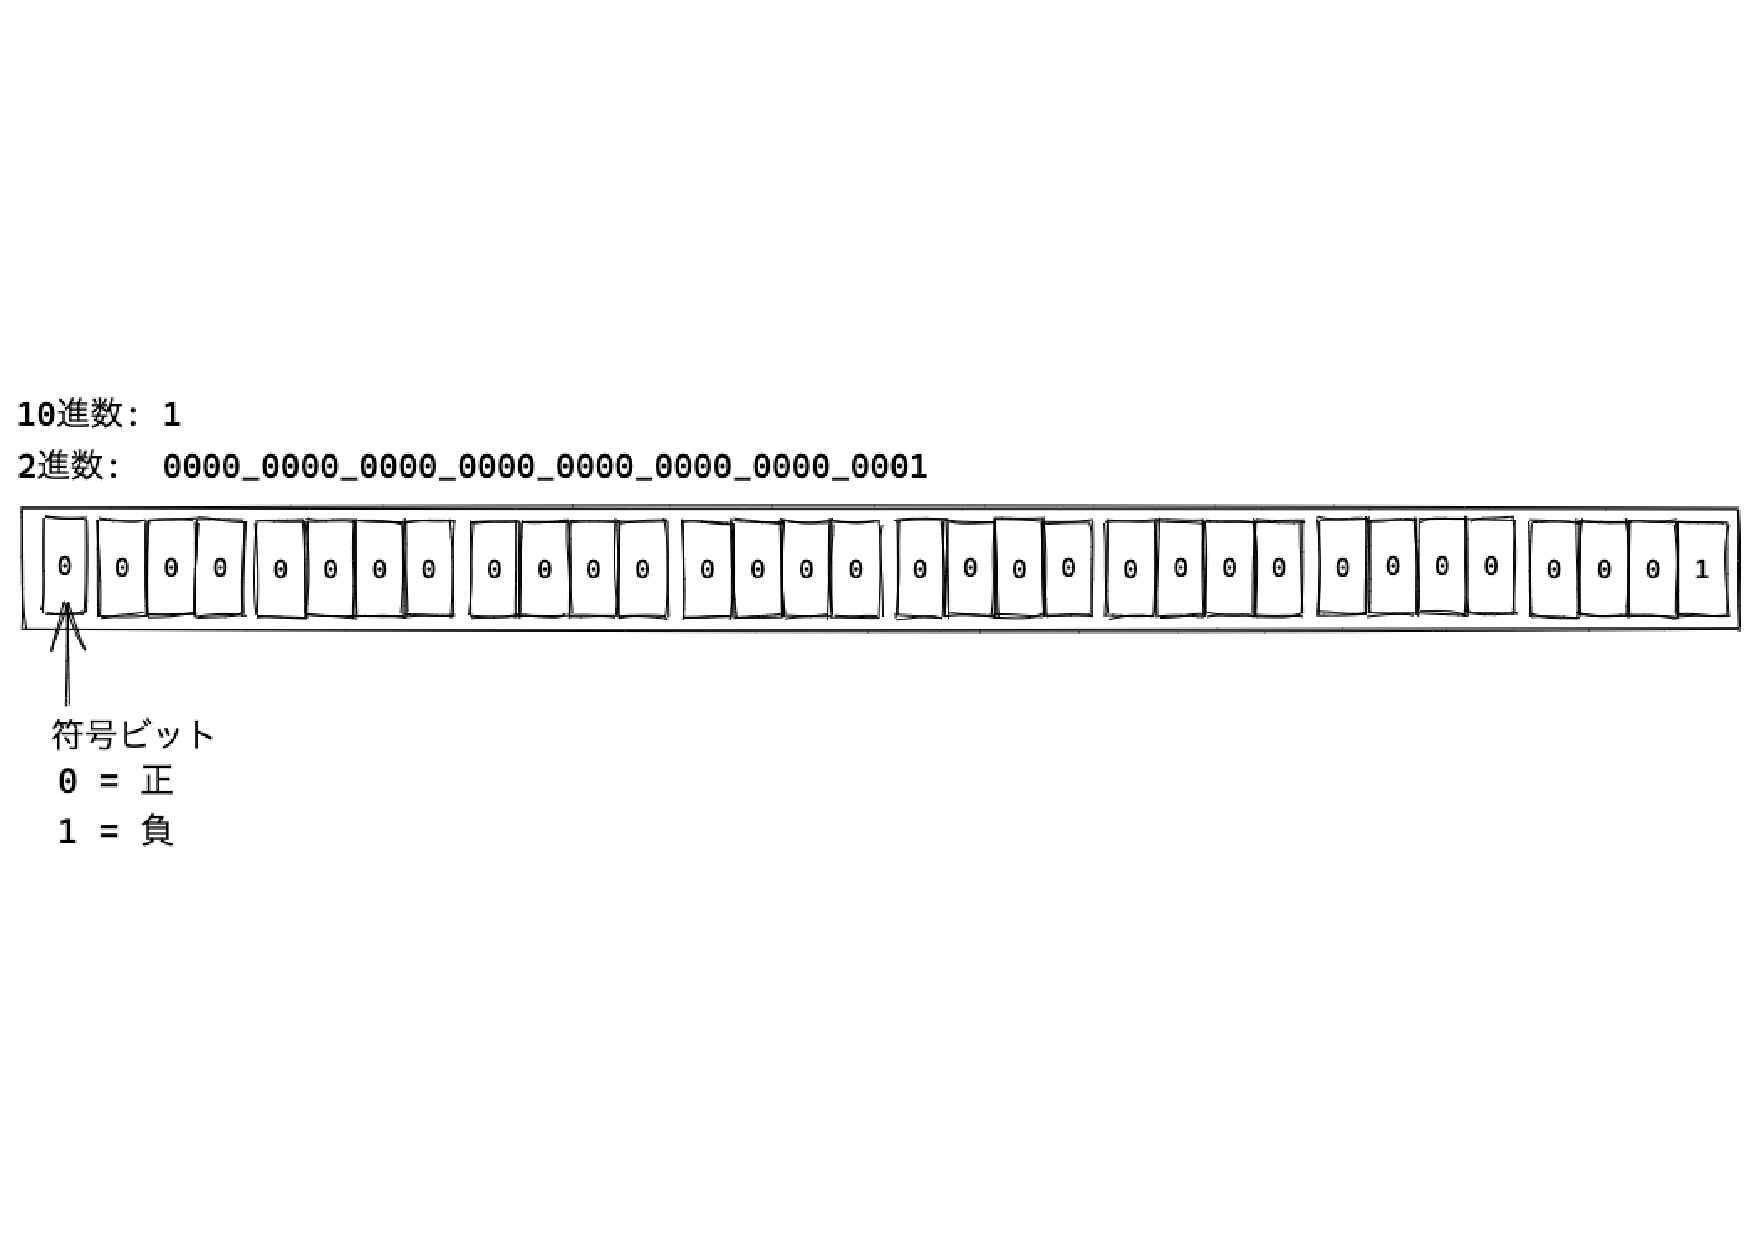
\includegraphics[width=130mm]{fig/0001.pdf}
\caption{1の符号付き32bit整数での表現}
\end{figure}

符号付き32ビット整数では負の数値は、2の補数形式という形式で表現されます。
2の補数とは、それぞれのビットを反転して1ビットを足した値となります。

たとえば、\texttt{-1}という数値の符号付き32ビット整数は、次のように2の補数で求められます。

\begin{itemize}
\item 10進数の\texttt{1}は、符号付き32ビット整数では\texttt{0000\_0000\_0000\_0000\_0000\_0000\_0000\_0001}となる
\item \texttt{0000\_0000\_0000\_0000\_0000\_0000\_0000\_0001}の各ビットを反転すると\texttt{1111\_1111\_1111\_1111\_1111\_1111\_1111\_1110}となる
\item これに1ビットを足すと\texttt{1111\_1111\_1111\_1111\_1111\_1111\_1111\_1111}となる
\end{itemize}

これによって、\texttt{-1}の符号付き32ビット整数は\texttt{1111\_1111\_1111\_1111\_1111\_1111\_1111\_1111}となります。

\begin{figure}[h]
\centering
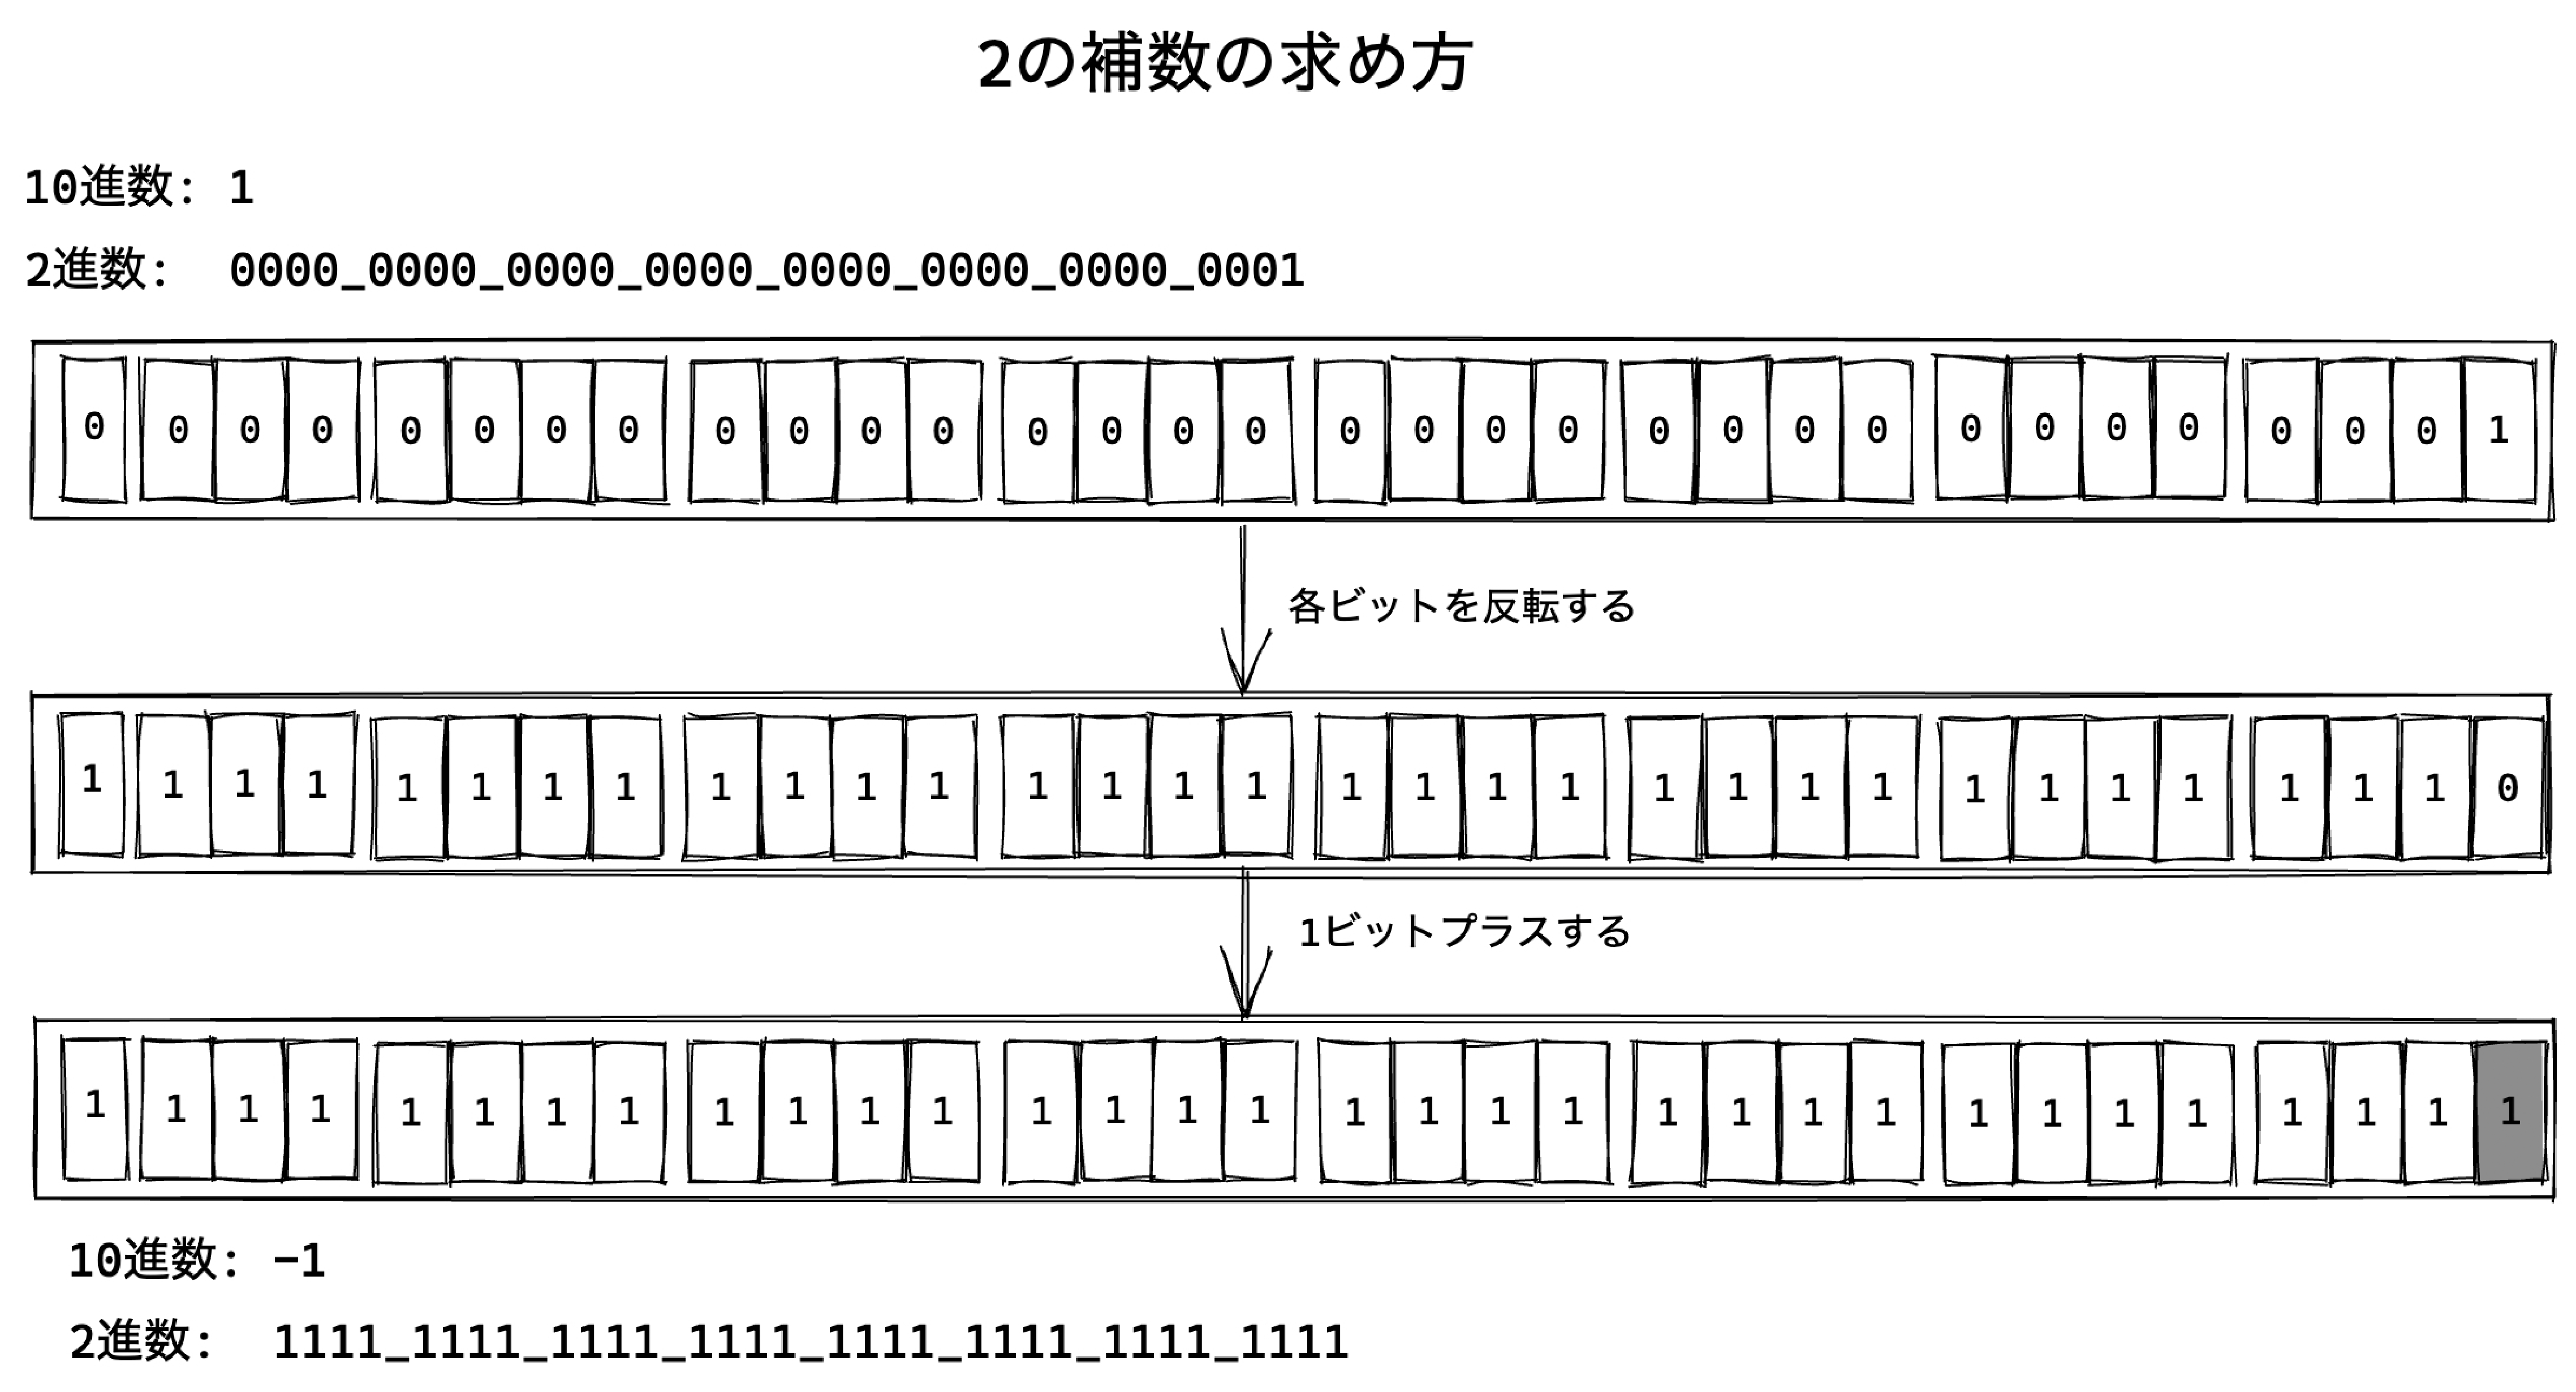
\includegraphics[width=130mm]{fig/1111.pdf}
\caption{-1の符号付き32ビット整数での表現}
\end{figure}

符号付き32ビット整数で表現できる数値の範囲は、\texttt{1000\_0000\_0000\_0000\_0000\_0000\_0000\_0000}から
\texttt{0111\_1111\_1111\_1111\_1111\_1111\_1111\_1111}までとなります。
10進数に直すと$-(2^{31})$(2の31乗の負の数)から$(2^{31}) - 1$(2の31乗から1引いた数)までとなります。
32ビットを超える数値については、32ビットをはみ出るビットが最上位(一番左)から順番に捨てられます。

これから見ていくビット演算子はオペランドを符号付き32ビット整数として扱い、その演算結果を10進数の数値として返します。

\hypertarget{bit-and}{%
\subsection{\texorpdfstring{ビット論理積(\texttt{\&})}{ビット論理積(\&)}}\label{bit-and}}\index{びっとろんりせき@ビット論理積}\index{&@\texttt{\&}}

ビット論理積演算子(\texttt{\&})はビットごとの\textbf{AND}\index{AND}演算した結果を返します。
AND演算では、オペランドの各ビットがどちらも\texttt{1}の場合は\texttt{1}となり、それ以外の場合は\texttt{0}となります。

次のコードでは、10進数の\texttt{15}と\texttt{9}をAND演算しています。
\texttt{15}は、符号付き32ビット整数では\texttt{0000\_0000\_0000\_0000\_0000\_0000\_0000\_1111}となります。
\texttt{9}は、符号付き32ビット整数では\texttt{0000\_0000\_0000\_0000\_0000\_0000\_0000\_1001}となります。
これらをAND演算した結果は\texttt{0000\_0000\_0000\_0000\_0000\_0000\_0000\_1001}となり、10進数の値である\texttt{9}を返します。

\begin{lstlisting}
console.log(15     & 9);      // => 9
// 同じ位の各ビット同士をAND演算する(上位の0は省略)
// 1111
// 1001
// ----
// 1001
console.log(0b1111 & 0b1001); // => 0b1001
\end{lstlisting}

\hypertarget{bit-or}{%
\subsection{\texorpdfstring{ビット論理和(\texttt{\textbar{}})}{ビット論理和(\textbar{})}}\label{bit-or}}\index{びっとろんりわ@ビット論理和}\index{\textbar{}@\texttt{\textbar{}}}

ビット論理和演算子(\texttt{\textbar{}})はビットごとの\textbf{OR}\index{OR}演算した結果を返します。
OR演算では、オペランドの各ビットがどちらか片方でも\texttt{1}の場合は\texttt{1}となり、両方とも\texttt{0}の場合は\texttt{0}となります。

\begin{lstlisting}
console.log(15     | 9);      // => 15
// 同じ位の各ビット同士をOR演算する(上位の0は省略)
// 1111
// 1001
// ----
// 1111
console.log(0b1111 | 0b1001); // => 0b1111
\end{lstlisting}

\hypertarget{bit-xor}{%
\subsection{\texorpdfstring{ビット排他的論理和(\texttt{\^{}})}{ビット排他的論理和(\^{})}}\label{bit-xor}}\index{びっとはいたてきろんりわ@ビット排他的論理和}\index{^@\texttt{\textasciicircum}}

ビット排他的論理和演算子(\texttt{\^{}})はビットごとの\textbf{XOR}\index{XOR}演算した結果を返します。
XOR演算では、オペランドのビットが異なるなら\texttt{1}、両方とも同じなら\texttt{0}となります。

\begin{lstlisting}
console.log(15     ^ 9);      // => 6
// 同じ位の各ビット同士をXOR演算する(上位の0は省略)
// 1111
// 1001
// ----
// 0110
console.log(0b1111 ^ 0b1001); // => 0b0110
\end{lstlisting}

\hypertarget{bit-not}{%
\subsection{\texorpdfstring{ビット否定(\texttt{\textasciitilde{}})}{ビット否定(\textasciitilde{})}}\label{bit-not}}\index{びっとひてい@ビット否定}\index{~@\texttt{\textasciitilde}}

単項演算子の否定演算子(\lstinline{~})はオペランドの各ビットを反転した値を返します。
これは1の補数として知られている値と同じものです。

次のコードでは、10進数で\texttt{15}を否定演算子(\lstinline{~})で各ビットを反転させた値を得ています。
\texttt{15}は\texttt{0000\_0000\_0000\_0000\_0000\_0000\_0000\_1111}です。
各ビットを反転させると\texttt{1111\_1111\_1111\_1111\_1111\_1111\_1111\_0000}となり、10進数では\texttt{-16}となります。

\begin{lstlisting}
console.log(~15); // => -16
\end{lstlisting}

\lstinline{~x}のように\texttt{x}をビット否定演算子で演算した結果は、\lstinline{-(x + 1)}となります。
この性質を利用する形で、ビット否定演算子(\lstinline{~})はビット演算以外でも使われていることがあります。

文字列(Stringオブジェクト)が持つ\texttt{indexOf}\index{indexOf@\texttt{indexOf}}メソッドは、マッチする文字列を見つけて、そのインデックス(位置)を返すメソッドです。
この\texttt{indexOf}メソッドは、検索対象が見つからない場合には\texttt{-1}を返します。

\begin{lstlisting}
const str = "森森本森森";
// 見つかった場合はインデックスを返す
// JavaScriptのインデックスは0から開始するので2を返す
console.log(str.indexOf("本")); // => 2
// 見つからない場合は-1を返す
console.log(str.indexOf("火")); // => -1
\end{lstlisting}

否定演算子(\lstinline{~})は1の補数を返すため、\lstinline{~(-1)}は\texttt{0}となります。

\begin{lstlisting}
console.log(~0); // => -1
console.log(~(-1)); // => 0
\end{lstlisting}

JavaScriptでは\texttt{0}も、if文では\texttt{false}として扱われます。
そのため、\lstinline{~indexOf}の結果が\texttt{0}となるのは、その文字列が見つからなかった場合だけとなります。
次のコードのように否定演算子(\lstinline{~})と\texttt{indexOf}メソッドを使ったイディオムが一部では使われていました。

\begin{lstlisting}
const str = "森森木森森";
// indexOfメソッドは見つからなかった場合は -1 を返す
if (str.indexOf("木") !== -1) {
    console.log("木を見つけました");
}
// 否定演算子(~)で同じ動作を実装
// (~(-1)) は 0 となるため、見つからなかった場合はif文の中身は実行されない
if (~str.indexOf("木")) {
    console.log("木を見つけました");
}
\end{lstlisting}

ES2015では、文字列(Stringオブジェクト)に\texttt{includes}\index{includes@\texttt{includes}}メソッドが実装されました。
\texttt{includes}メソッドは指定した文字列が含まれているかを真偽値で返します。

\begin{lstlisting}
const str = "森森木森森";
if (str.includes("木")) {
    console.log("木を見つけました");
}
\end{lstlisting}

そのため、否定演算子(\lstinline{~})と\texttt{indexOf}メソッドを使ったイディオムは、\texttt{includes}メソッドに置き換えられます。

\hypertarget{left-shift}{%
\subsection{\texorpdfstring{左シフト演算子(\texttt{\textless{}\textless{}})}{左シフト演算子(\textless{}\textless{})}}\label{left-shift}}\index{ひだりしふとえんざんし@左シフト演算子}\index{<<@\texttt{\textless{}\textless{}}}

左シフト演算子は、数値である\texttt{num}を\texttt{bit}の数だけ左へシフトします。
左にあふれたビットは破棄され、\texttt{0}のビットを右から詰めます。

\begin{lstlisting}
num << bit;
\end{lstlisting}

次のコードでは、\texttt{9}を2ビット分だけ左へシフトしています。

\begin{lstlisting}
console.log(     9 << 2); // => 36
console.log(0b1001 << 2); // => 0b10_0100
\end{lstlisting}

\hypertarget{right-shift}{%
\subsection{\texorpdfstring{右シフト演算子(\texttt{\textgreater{}\textgreater{}})}{右シフト演算子(\textgreater{}\textgreater{})}}\label{right-shift}}\index{みぎしふとえんざんし@右シフト演算子}\index{>>@\texttt{\textgreater{}\textgreater{}}}

右シフト演算子は、数値である\texttt{num}を\texttt{bit}の数だけ右へシフトします。
右にあふれたビットは破棄され、左端のビットのコピーを左から詰めます。

\begin{lstlisting}
num >> bit;
\end{lstlisting}

次のコードでは、\texttt{-9}を2ビット分だけ右へシフトしています。
左端のビットのコピーを使うため、常に符号は維持されます。

\begin{lstlisting}
console.log((-9) >> 2); // => -3
//    1111_1111_1111_1111_1111_1111_1111_0111 >> 2
// => 1111_1111_1111_1111_1111_1111_1111_1101
\end{lstlisting}

\hypertarget{fill-zero-right-shift}{%
\subsection{\texorpdfstring{ゼロ埋め右シフト演算子(\texttt{\textgreater{}\textgreater{}\textgreater{}})}{ゼロ埋め右シフト演算子(\textgreater{}\textgreater{}\textgreater{})}}\label{fill-zero-right-shift}}\index{ぜろうめみぎしふとえんざんし@ゼロ埋め右シフト演算子}\index{>>>@\texttt{\textgreater{}\textgreater{}\textgreater{}}}

ゼロ埋め右シフト演算子は、数値である\texttt{num}を\texttt{bit}の数だけ右へシフトするのは右シフト演算子(\lstinline{>>})と同じです。
異なる点としては右にあふれたビットは破棄され、\texttt{0}のビットを左から詰めます。

次のコードでは、\texttt{-9}を2ビット分だけゼロ埋め右シフトしています。
左端のビットは\texttt{0}となるため、常に正の値となります。

\begin{lstlisting}
console.log((-9) >>> 2); // => 1073741821
//    1111_1111_1111_1111_1111_1111_1111_0111 >>> 2
// => 0011_1111_1111_1111_1111_1111_1111_1101
\end{lstlisting}

\hypertarget{assignment-operator}{%
\section{\texorpdfstring{代入演算子(\texttt{=})}{代入演算子(=)}}\label{assignment-operator}}\index{だいにゅうえんざんし@代入演算子}\index{=@\texttt{=}}

代入演算子(\texttt{=})は変数に対して値を代入します。
代入演算子については「\hyperlink{variable-and-declaration}{変数と宣言}」の章も参照してください。

\begin{lstlisting}
let x = 1;
x = 42;
console.log(x); // => 42
\end{lstlisting}

また、代入演算子は二項演算子と組み合わせて利用できます。
\lstinline{+=}、\lstinline{-=}、\lstinline{*=}、\lstinline{/=}、\lstinline{%=}、\lstinline{<<=}、\lstinline{>>=}、\lstinline{>>>=}、\lstinline{&=}、\lstinline{^=}、\lstinline{|=}、\lstinline{**=}のように、演算した結果を代入できます。

\begin{lstlisting}
let num = 1;
num += 10; // num = num + 10; と同じ
console.log(num); // => 11
\end{lstlisting}

\hypertarget{destructuring-assignment}{%
\subsection[分割代入(Destructuring
assignment)]{分割代入(Destructuring
assignment)\protect\icon{fig/es2015.eps}}\label{destructuring-assignment}}\index{ぶんかつだいにゅう@分割代入}\index{Destructuring assignment}

今まで見てきた代入演算子は1つの変数に値を代入するものでした。
分割代入を使うことで、配列やオブジェクトの値を複数の変数へ同時に代入できます。
分割代入は短縮記法のひとつでES2015から導入された構文です。

分割代入は、代入演算子(\texttt{=})を使うのは同じですが、左辺のオペランドが配列リテラルやオブジェクトリテラルとなります。

次のコードでは、右辺の配列の値を、左辺の配列リテラルの対応するインデックスに書かれた変数名へ代入します。

\begin{lstlisting}
const array = [1, 2];
// aにはarrayの0番目の値、bには1番目の値が代入される
const [a, b] = array;
console.log(a); // => 1
console.log(b); // => 2
\end{lstlisting}

これは、次のように書いたのと同じ結果になります。

\begin{lstlisting}
const array = [1, 2];
const a = array[0];
const b = array[1];
\end{lstlisting}

同様にオブジェクトも分割代入に対応しています。
オブジェクトの場合は、右辺のオブジェクトのプロパティ値を、左辺に対応するプロパティ名へ代入します。

\begin{lstlisting}
const obj = {
    "key": "value"
};
// プロパティ名keyの値を、変数keyとして定義する
const { key } = obj;
console.log(key); // => "value"
\end{lstlisting}

これは、次のように書いたのと同じ結果になります。

\begin{lstlisting}
const obj = {
    "key": "value"
};
const key = obj.key;
\end{lstlisting}

\hypertarget{logical-operator}{%
\section{論理演算子\index{ろんりえんざんし@論理演算子}}\label{logical-operator}}

論理演算子は基本的に真偽値を扱う演算子でAND(かつ)、OR(または)、NOT(否定)を表現できます。

\hypertarget{and-operator}{%
\subsection{AND演算子(\texttt{\&\&})\index{ANDえんざんし(\&\&)@AND演算子(\texttt{\&\&})}}\label{and-operator}}

AND演算子(\texttt{\&\&})は、左辺の値の評価結果が\texttt{true}ならば、右辺の評価結果を返します。
一方で、左辺の値の評価結果が\texttt{false}ならば、そのまま左辺の値を返します。

\begin{lstlisting}
// 左辺はtrueであるため、右辺の評価結果を返す
console.log(true && "右辺の値"); // => "右辺の値"
// 左辺がfalseであるなら、その時点でfalseを返す
// 右辺は評価されない
console.log(false && "右辺の値"); // => false
\end{lstlisting}

AND演算子(\texttt{\&\&})は、左辺の評価が\texttt{false}の場合、オペランドの右辺は評価されません。
次のように、左辺が\texttt{false}の場合は、右辺に書いた\texttt{console.log}関数自体が実行されません。

\begin{lstlisting}
// 左辺がtrueなので、右辺は評価される
true && console.log("このコンソールログは実行されます");
// 左辺がfalseなので、右辺は評価されない
false && console.log("このコンソールログは実行されません");
\end{lstlisting}

このような値が決まった時点でそれ以上評価しないことを\textbf{\textgt{短絡評価}}と呼びます。

また、AND演算子は左辺を評価する際に、左辺を真偽値へと\hyperlink{implicit-coercion}{暗黙的な型変換}をしてから判定します。
真偽値への暗黙的な型変換では、次に挙げる値は\texttt{false}へ変換されます。

\begin{itemize}
\item \texttt{false}
\item \texttt{undefined}
\item \texttt{null}
\item \texttt{0}
\item \texttt{0n}
\item \texttt{NaN}
\item \texttt{""}(空文字列)
\end{itemize}

暗黙的な型変換によって\texttt{false}に変換されるこれらの値をまとめて\textbf{falsy}な値と呼びます。
falsyではない値は、\texttt{true}へと変換されます。
\texttt{true}へと変換される値の種類は多いため、\texttt{false}へと変換されない値は\texttt{true}となることは覚えておくとよいです。
このオペランドを真偽値に変換してから評価するのはAND、OR、NOT演算子で共通の動作です。

次のように、AND演算子(\texttt{\&\&})は左辺を真偽値へと変換した結果が\texttt{true}の場合に、右辺の評価結果を返します。
つまり、左辺がfalsyの場合は、右辺は評価されません。

\begin{lstlisting}
// 左辺はfalsyではないため、評価結果として右辺を返す
console.log("文字列" && "右辺の値"); // => "右辺の値"
console.log(42 && "右辺の値"); // => "右辺の値"
// 左辺がfalsyであるため、評価結果として左辺を返す
console.log("" && "右辺の値"); // => ""
console.log(0 && "右辺の値"); // => 0
console.log(null && "右辺の値"); // => null
\end{lstlisting}

AND演算子は、if文と組み合わせて利用することが多い演算子です。

次のように、\texttt{value}がString型で\textbf{\textgt{かつ}}値が\texttt{"str"}である場合という条件をひとつの式として書くことができます。

\begin{lstlisting}
const value = "str";
if (typeof value === "string" && value === "str") {
    console.log(`${value} is string value`);
}
// if文のネストで書いた場合と結果は同じとなる
if (typeof value === "string") {
    if (value === "str") {
        console.log(`${value} is string value`);
    }
}
\end{lstlisting}

このときに、\texttt{value}がString型でない場合は、その時点でif文の条件式は\texttt{false}となります。
そのため、\texttt{value}がString型ではない場合は、AND演算子(\texttt{\&\&})の右辺は評価されずに、if文の中身も実行されません。

AND演算子(\texttt{\&\&})を使うと、if文のネストに比べて短く書くことができます。

しかし、if文が3重4重にネストしているのは複雑なのと同様に、
AND演算子やOR演算子が3つ4つ連続すると複雑で読みにくいコードとなります。
その場合は抽象化ができないかを検討するべきサインとなります。

\hypertarget{or-operator}{%
\subsection{OR演算子(\texttt{||})\index{ORえんざんし(||)@OR演算子(\texttt{||})}}\label{or-operator}}

OR演算子(\texttt{||})は、左辺の値の評価結果が\texttt{true}ならば、そのまま左辺の値を返します。
一方で、左辺の値の評価結果が\texttt{false}であるならば、右辺の評価結果を返します。

\begin{lstlisting}
// 左辺がtrueなので、左辺の値が返される
console.log(true || "右辺の値"); // => true
// 左辺がfalseなので、右辺の値が返される
console.log(false || "右辺の値"); // => "右辺の値"
\end{lstlisting}

OR演算子(\texttt{||})は、左辺の評価が\texttt{true}の場合、オペランドの右辺を評価しません。
これは、AND演算子(\texttt{\&\&})と同様の短絡評価となるためです。

\begin{lstlisting}
// 左辺がtrueなので、右辺は評価されない
true || console.log("このコンソールログは実行されません");
// 左辺がfalseなので、右辺は評価される
false || console.log("このコンソールログは実行されます");
\end{lstlisting}

また、OR演算子は左辺を評価する際に、左辺を真偽値へと暗黙的な型変換をします。
次のように、OR演算子は左辺がfalsyの場合には右辺の値を返します。

\begin{lstlisting}
// 左辺がfalsyなので、右辺の値が返される
console.log(0 || "左辺はfalsy"); // => "左辺はfalsy"
console.log("" || "左辺はfalsy"); // => "左辺はfalsy"
console.log(null || "左辺はfalsy"); // => "左辺はfalsy"
// 左辺はfalsyではないため、左辺の値が返される
console.log(42 || "右辺の値"); // => 42
console.log("文字列" || "右辺の値"); // => "文字列"
\end{lstlisting}

OR演算子は、if文と組み合わせて利用することが多い演算子です。

次のように、\texttt{value}が\texttt{0}\textbf{\textgt{または}}\texttt{1}の場合にif文の中身が実行されます。

\begin{lstlisting}
const value = 1;
if (value === 0 || value === 1) {
    console.log("valueは0または1です。");
}
\end{lstlisting}

\hypertarget{not-operator}{%
\subsection{NOT演算子(\texttt{!})\index{NOTえんざんし(!)@NOT演算子(\texttt{!})}}\label{not-operator}}

NOT演算子(\texttt{!})は、\texttt{オペランド}の評価結果が\texttt{true}ならば、\texttt{false}を返します。
一方で、\texttt{オペランド}の評価結果が\texttt{false}ならば、\texttt{true}を返します。
つまり、オペランドの評価結果を反転した真偽値を返します。

\begin{lstlisting}
console.log(!false); // => true
console.log(!true);  // => false
\end{lstlisting}

NOT演算子(\texttt{!})もAND演算子(\texttt{\&\&})とOR演算子(\texttt{||})と同様に真偽値へと\hyperlink{implicit-coercion}{暗黙的な型変換}します。
falsyである値は\texttt{true}へ変換され、falsyではない値は\texttt{false}へと変換されます。

\begin{lstlisting}
// falsyな値はtrueとなる
console.log(!0); // => true
console.log(!""); // => true
console.log(!null); // => true
// falsyではない値はfalseとなる
console.log(!42);  // => false
console.log(!"文字列");  // => false
\end{lstlisting}

NOT演算子は必ず真偽値を返すため、次のように2つNOT演算子を重ねて真偽値へ変換するという使い方も見かけます。
たとえば、\texttt{!!falsyな値}のように2度反転すれば\texttt{false}になります。

\begin{lstlisting}
const str = "";
// 空文字列はfalsyであるため、true -> falseへと変換される
console.log(!!str); // => false
\end{lstlisting}

このようなケースの多くは、比較演算子を使うなどより明示的な方法で、真偽値を得ることができます。
安易に\texttt{!!}による変換に頼るよりは別の方法を探してみるのがいいでしょう。

\begin{lstlisting}
const str = "";
// 空文字列(長さが0より大きな文字列)でないことを判定
console.log(str.length > 0); // => false
\end{lstlisting}

\hypertarget{nullish-coalescing-operator}{%
\section{Nullish coalescing演算子(\texttt{??})\index{Nullish coalescingえんざんし(??)@Nullish coalescing演算子(\texttt{??})}\,\protect\icon{fig/es2020.eps}}\label{nullish-coalescing-operator}}

Nullish coalescing演算子(\texttt{??})は、左辺の値が\textbf{nullish}であるならば、右辺の評価結果を返します。
\textbf{nullish}とは、評価結果が\texttt{null}または\texttt{undefined}となる値のことです。

\begin{lstlisting}
// 左辺がnullishであるため、右辺の値の評価結果を返す
console.log(null ?? "右辺の値"); // => "右辺の値"
console.log(undefined ?? "右辺の値"); // => "右辺の値"
// 左辺がnullishではないため、左辺の値の評価結果を返す
console.log(true ?? "右辺の値"); // => true
console.log(false ?? "右辺の値"); // => false
console.log(0 ?? "右辺の値"); // => 0
console.log("文字列" ?? "右辺の値"); // => "文字列"
\end{lstlisting}

Nullish coalescing演算子(\texttt{??})とOR演算子(\texttt{||})は、値のデフォルト値を指定する場合によく利用されています。
OR演算子(\texttt{||})は左辺がfalsyの場合に右辺を評価するため、意図しない結果となる場合があります。

次のコードは、\texttt{inputValue}が未定義だった場合に、\texttt{value}に対するデフォルト値をOR演算子(\texttt{||})で指定しています。
\texttt{inputValue}が未定義(\texttt{undefined})の場合は、意図したようにOR演算子(\texttt{||})の右辺で指定した\texttt{42}が入ります。
しかし、\texttt{inputValue}が\texttt{0}という値であった場合は、\texttt{0}はfalsyであるため\texttt{value}には右辺の\texttt{42}が入ります。
これでは\texttt{0}という値が扱えないため、意図しない動作となっています。

\begin{lstlisting}
const inputValue = 任意の値または未定義;
// inputValueがfalsyの場合は、valueには42が入る
// inputValueが0の場合は、valueに42が入ってしまう
const value = inputValue || 42;
console.log(value);
\end{lstlisting}

この問題を解決するためにES2020でNullish coalescing演算子(\texttt{??})が導入されています。

Nullish coalescing演算子(\texttt{??})では、左辺がnullishの場合のみ、\texttt{value}に右辺で指定した\texttt{42}が入ります。
そのため、\texttt{inputValue}が\texttt{0}という値が入った場合は、\texttt{value}にはそのまま\texttt{inputValue}の値である\texttt{0}が入ります。

\begin{lstlisting}
const inputValue = 任意の値または未定義;
// inputValueがnullishの場合は、valueには42が入る
// inputValueが0の場合は、valueに0が入る
const value = inputValue ?? 42;
console.log(value);
\end{lstlisting}

\hypertarget{ternary-operator}{%
\section{\texorpdfstring{条件(三項)演算子(\texttt{?}と\texttt{:})}{条件(三項)演算子(?と:)}}\label{ternary-operator}}\index{?@\texttt{?}}\index{:@\texttt{:}}

条件演算子(\texttt{?}と\texttt{:})は三項をとる演算子であるため、三項演算子\index{さんこうえんざんし@三項演算子}とも呼ばれます。

条件演算子は\texttt{条件式}\index{じょうけんしき@条件式}を評価した結果が\texttt{true}ならば、\texttt{Trueのとき処理する式}の評価結果を返します。
\texttt{条件式}が\texttt{false}である場合は、\texttt{Falseのとき処理する式}の評価結果を返します。

\begin{lstlisting}
条件式 ? Trueのとき処理する式 : Falseのとき処理する式;
\end{lstlisting}

if文との違いは、条件演算子は式として書くことができるため値を返すという点です。
たとえば、次のように\texttt{条件式}の評価結果により\texttt{"A"}または\texttt{"B"}どちらかを返します。

\begin{lstlisting}
const valueA = true ? "A" : "B";
console.log(valueA); // => "A"
const valueB = false ? "A" : "B";
console.log(valueB); // => "B"
\end{lstlisting}

条件分岐による値を返せるため、条件によって変数の初期値が違う場合などに使われます。

次の例では、\texttt{text}文字列に\texttt{prefix}となる文字列を先頭につける関数を書いています。
第二引数の\texttt{prefix}を省略したり文字列ではないものが指定された場合に、デフォルトの\texttt{prefix}を使います。
第二引数が省略された場合には、\texttt{prefix}に\texttt{undefined}が入ります。

条件演算子の評価結果は値を返すので、\texttt{const}を使って宣言と同時に代入できます。

\begin{lstlisting}
function addPrefix(text, prefix) {
    // prefixが指定されていない場合は"デフォルト:"を付ける
    const pre = typeof prefix === "string" ? prefix : "デフォルト:";
    return pre + text;
}

console.log(addPrefix("文字列")); // => "デフォルト:文字列"
console.log(addPrefix("文字列", "カスタム:")); // => "カスタム:文字列"
\end{lstlisting}

if文を使った場合は、宣言と代入を分ける必要があるため、\texttt{const}を使うことができません。

\begin{lstlisting}
function addPrefix(text, prefix) {
    let pre = "デフォルト:";
    if (typeof prefix === "string") {
        pre = prefix;
    }
    return pre + text;
}

console.log(addPrefix("文字列")); // => "デフォルト:文字列"
console.log(addPrefix("文字列", "カスタム:")); // => "カスタム:文字列"
\end{lstlisting}


\hypertarget{group-operator}{%
\subsection{\texorpdfstring{グループ化演算子(\texttt{(}と\texttt{)})}{グループ化演算子((と))}}\label{group-operator}}\index{ぐるーぷかえんざんし@グループ化演算子}\index{()@\texttt{()}}

グループ化演算子は複数の二項演算子が組み合わさった場合に、演算子の優先順位を明示できる演算子です。

たとえば、次のようにグループ化演算子で囲んだ部分が最初に処理されるため、結果も変化します。

\begin{lstlisting}
const a = 1;
const b = 2;
const c = 3;
console.log(a + b * c); // => 7
console.log((a + b) * c); // => 9
\end{lstlisting}

\href{https://developer.mozilla.org/ja/docs/Web/JavaScript/Reference/Operators/Operator_Precedence\#Table}{演算子の優先順位}\footnote{\url{https://developer.mozilla.org/ja/docs/Web/JavaScript/Reference/Operators/Operator_Precedence\#Table}}はECMAScript仕様で定義されていますが、演算子の優先度をすべて覚えるのは難しいです。
演算子の優先順位\index{えんざんし@演算子!ゆうせんじゅんい@優先順位}の中でもグループ化演算子は優先順位が高く、グループ化演算子を使うことによって優先順位を明示できます。

次のようなグループ化演算子を使わずに書いたコードを見てみましょう。
\texttt{x}が\texttt{true}または、\texttt{y}かつ\texttt{z}が\texttt{true}であるときに処理されます。

\begin{lstlisting}
if (x || y && z) {
    // x が true または
    // y かつ z が true
}
\end{lstlisting}

ひとつの式に複数の種類の演算子が出てくると読みにくくなる傾向があります。
このような場合にはグループ化演算子を使い、結合順を明示して書くようにしましょう。

\begin{lstlisting}
if (x || (y && z)) {
    // x が true または
    // y かつ z が true
}
\end{lstlisting}

しかし、ひとつの式で多数の演算をするよりも、式自体を分けたほうが読みやすい場合もあります。

次のように\texttt{a}と\texttt{b}が文字列型
または
\texttt{x}と\texttt{y}が数値型の場合に処理するif文を考えてみます。
グループ化演算子を使い、そのまま1つの条件式で書くことも可能ですが、読みにくくなってしまいます。

\begin{lstlisting}
if ((typeof a === "string" && typeof b === "string") || (typeof x === "number"
 && typeof y === "number")) {
    // aとbが文字列型 または
    // xとyが数値型
}
\end{lstlisting}

このように無理して1つの式(1行)で書くよりも、条件式を分解してそれぞれの結果を変数として定義したほうが読みやすくなる場合もあります。

\begin{lstlisting}
const isAbString = typeof a === "string" && typeof b === "string";
const isXyNumber = typeof x === "number" && typeof y === "number";
if (isAbString || isXyNumber) {
    // aとbが文字列型 または
    // xとyが数値型
}
\end{lstlisting}

そのため、グループ化演算子ですべての条件をまとめるのではなく、
それぞれの条件を分解して名前をつける(変数として定義する)ことも重要です。

\hypertarget{comma-operator}{%
\section{\texorpdfstring{カンマ演算子(\texttt{,})}{カンマ演算子(,)}}\label{comma-operator}}\index{かんまえんざんし@カンマ演算子}\index{,@\texttt{,}}

カンマ演算子(\texttt{,})は、カンマ(\texttt{,})で区切った式を左から順に評価し、
最後の式の評価結果を返します。

次の例では、\texttt{式1}、\texttt{式2}、\texttt{式3}の順に評価され、\texttt{式3}の評価結果を返します。

\begin{lstlisting}
式1, 式2, 式3;
\end{lstlisting}

これまでに、カンマで区切るという表現は、\texttt{const}による変数宣言などでも出てきました。
左から順に実行する点ではカンマ演算子の挙動は同じものですが、構文としては似て非なるものです。

\begin{lstlisting}
const a = 1, b = 2, c = a + b;
console.log(c); // => 3
\end{lstlisting}

一般にカンマ演算子を利用する機会はほとんどないため、「カンマで区切った式は左から順に評価される」ということだけを知っていれば問題ありません\footnote{カンマ演算子を活用したテクニックとしてindirect
  call\index{indirect
  call}というものがあります。\url{https://2ality.com/2014/01/eval.html}}。

\hypertarget{conclusion}{%
\section{まとめ}\label{conclusion}}

この章では演算子について学びました。

\begin{itemize}
\item
  演算子はよく利用する演算処理を記号などで表現したもの
\item
  四則演算や論理演算などさまざまな種類の演算子がある
\item
  演算子には優先順位が定義されており、グループ化演算子で明示できる
\end{itemize}
